\section{Monoalfabetici}

	\begin{frame}
		\begin{center}
			\LARGE{\textcolor{blue}{Cifrari a sostituzione monoalfabetici}}
		\end{center}
	\end{frame}

	\subsection{Intro}
		
		\begin{frame}
			\frametitle{Shift Encryption}		
			\begin{itemize}
				\item La \textcolor{blue}{encryption} viene eseguita lettera per lettera
				\item Ogni lettera viene sostituita con un'altra lettera (\tblue{fissata})
				\item Identifichiamo le lettere con i \textcolor{blue}{numeri} da 0 a 25 (A=0, B=1, ecc)
				\item Chiamiamo K la chiave segreta che sarà un \textcolor{blue}{numero} compreso tra 1 e 25
				\item Le \textcolor{blue}{funzioni di encryption e decryption} saranno le seguenti
					$$\begin{cases}
						c = E_K[p] = (p+K) mod 26 \\
						p = D_K[c] = (c-K) mod 26
					\end{cases}$$
			\end{itemize}
		\end{frame}
		
		\begin{frame}
			\frametitle{Substitution Encryption}		
			\begin{itemize}
				\item \tblue{Facilmente attaccabile} con forza bruta (solo 26 chiavi possibili)
				\item Si risolve utilizzando una \textcolor{blue}{qualunque} permutazione delle lettere (si passa a 26! $\approx 4x10^{26}$ combinazioni)
				\item Nuovo problema: \tblue{analisi delle frequenze}
			\end{itemize}
		\end{frame}
		
		\begin{frame}
			\frametitle{Criptanalisi}		
			\begin{itemize}
				\item Nella lingua italiana le 5 lettere \textcolor{blue}{più frequenti} sono E($12.62\%$), I($11.62\%$), A($10.41\%$), O($8.71\%$) e R($6.70\%$)
				\item Se si ha a disposizione \textcolor{blue}{abbastanza} ciphertext, la frequenza delle lettere che appaiono in questo sarà più o meno la stessa
				\item Si prova a sostituire le lettere del ciphertext con le  lettere che hanno circa la stessa frequenza e con \tblue{pochi} tentativi si trova il plaintext (e la rispettiva \tblue{chiave})
				\item Vediamo un \tblue{esempio}
			\end{itemize}
		\end{frame}
	
		{
			\setbeamercolor{background canvas}{bg=}
			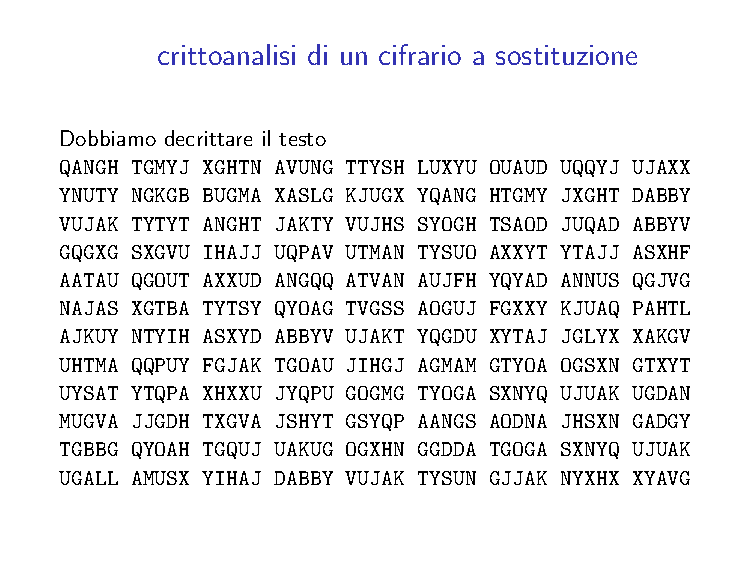
\includepdf[pages={-}]{esempi/cesare.pdf}
		}
					
		\begin{frame}
			\frametitle{Soluzione}		
			\begin{itemize}
				\item Criptare più lettere alla volta (\tblue{cifrari monoalfabetici a blocchi})
				\item Usare più cifrari monoalfabetici a rotazione (\tblue{cifrari polialfabetici})
			\end{itemize}
		\end{frame}
		
	\subsection{Hill}
		
		\begin{frame}
			\begin{center}
				\LARGE{\textcolor{blue}{Cifrari monoalfabetici a blocchi}}
			\end{center}
		\end{frame}
		
		\begin{frame}
			\frametitle{Cenni preliminari}		
			\begin{itemize}
				\item Si lavora con \tblue{\emph{q-grammi}}
				\item La distribuzione dei q-grammi è molto più \tblue{piatta}
				\item Serve \tblue{molto più ciphertext} per effettuare un'analisi delle frequenze significativa
				\item Il cifrario principale in questa categoria è il cifrario di Hill
			\end{itemize}
		\end{frame}
		
		\begin{frame}
			\frametitle{Cifrario di Hill}
			\begin{columns}
				\begin{column}{0.4\textwidth}
					\begin{center}
						\begin{figure}
							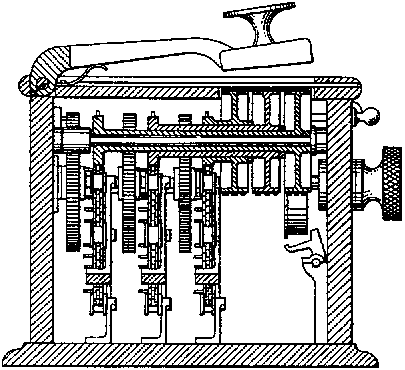
\includegraphics[width=\columnwidth]{img/Hill.png}
							\caption{Macchina cifrante con cifrario di Hill (tratta dal brevetto)}
						\end{figure}	
					\end{center}
				\end{column}
				\begin{column}{0.6\textwidth}
					\begin{itemize}
						\item Creato da \tblue{Lester S. Hill} nel 1929
						\item Si basa sull'utilizzo di \tblue{matrici} e \tblue{algebra modulare}
						\item Si considerano \emph{m} lettere alla volta $p_1,p_2,\dots,p_m$ con \emph{m} \tblue{fissato}.
					\end{itemize}
				\end{column}
			\end{columns}	
		\end{frame}
		
		\begin{frame}
			\frametitle{Encryption}	
			Definiamo:
			$$C = 
			\left(\begin{matrix}
			c_1\\
			\vdots\\
			c_m
			\end{matrix}\right),
			K = 
			\left[\begin{matrix}
			k_{11} & \dots & k_{1m}\\
			\vdots & \vdots & \vdots\\
			k_{m1} & \dots & k_{mm}\\
			\end{matrix}\right],
			P = 
			\left(\begin{matrix}
			p_1\\
			\vdots\\
			p_m
			\end{matrix}\right)$$
			La sostituzione è ottenuta risolvendo il sistema di equazioni lineari:
			$$\begin{cases}
				c_1 = (k_{11}\cdot p_1 + \dots + k_{1m}\cdot p_m)mod 26\\
				\vdots\\
				c_m = (k_{m1}\cdot p_1 + \dots + k_{mm}\cdot p_m)mod 26
			\end{cases}$$	
			In forma matriciale:
			$$E_K[P] = C = KxP$$
		\end{frame}
		
		\begin{frame}
			\frametitle{Decryption}	
			Dal ciphertext si ritorna al plaintext con la formula inversa:
			$$D_K[C] = K^{-1}xC = K^{-1}xKxP = P$$
			Per questo motivo $K$ deve essere \tblue{invertibile} modulo 26.
			\begin{block}{}
				Si sfrutta il principio della \tblue{diffusione} che richiede che ogni lettera del ciphertext dipenda da tutte le lettere del plaintext cosicché le singole lettere del ciphertext non possano essere analizzate singolarmente.
			\end{block}
		\end{frame}
		
		\begin{frame}
			\frametitle{Attacco}	
			Hill è \tblue{vulnerabile} ad un attacco \tblue{known plaintext}.
			
			L'attaccante ha bisogno di \emph{m} coppie di plaintext e rispettivo ciphertext.
			$$\begin{matrix}
				\langle P_1,C_1\rangle & dove \ C_1 = KxP_1\\
				\vdots & \vdots\\
				\langle P_m,C_m\rangle & dove \ C_m = KxP_m
			\end{matrix}$$
			Crea le due matrici 
			$$P^* = \left[P_1|\dots|P_m\right]$$
			$$C^* = \left[C_1|\dots|C_m\right]$$ 
		\end{frame}
		
		\begin{frame}
			\frametitle{Attacco}	
			Sapendo che
			$$C^* = KxP^*(mod 26)$$
			Se $P^*$ è invertibile, calcola l'inversa e può trovare la chiave $K$
			$$C^*xP^{*-1} = KxP^*xP^{*-1} = K$$
			facendo cadere tutto il cifrario.
			Se non lo è, tutto quello che deve fare è raccogliere altre coppie plaintext, ciphertext.
		\end{frame}